% Figures for the fixed bidding rules (analyze/fixed_rules_analysis.py).
\begin{figure}[H]
    \centering
    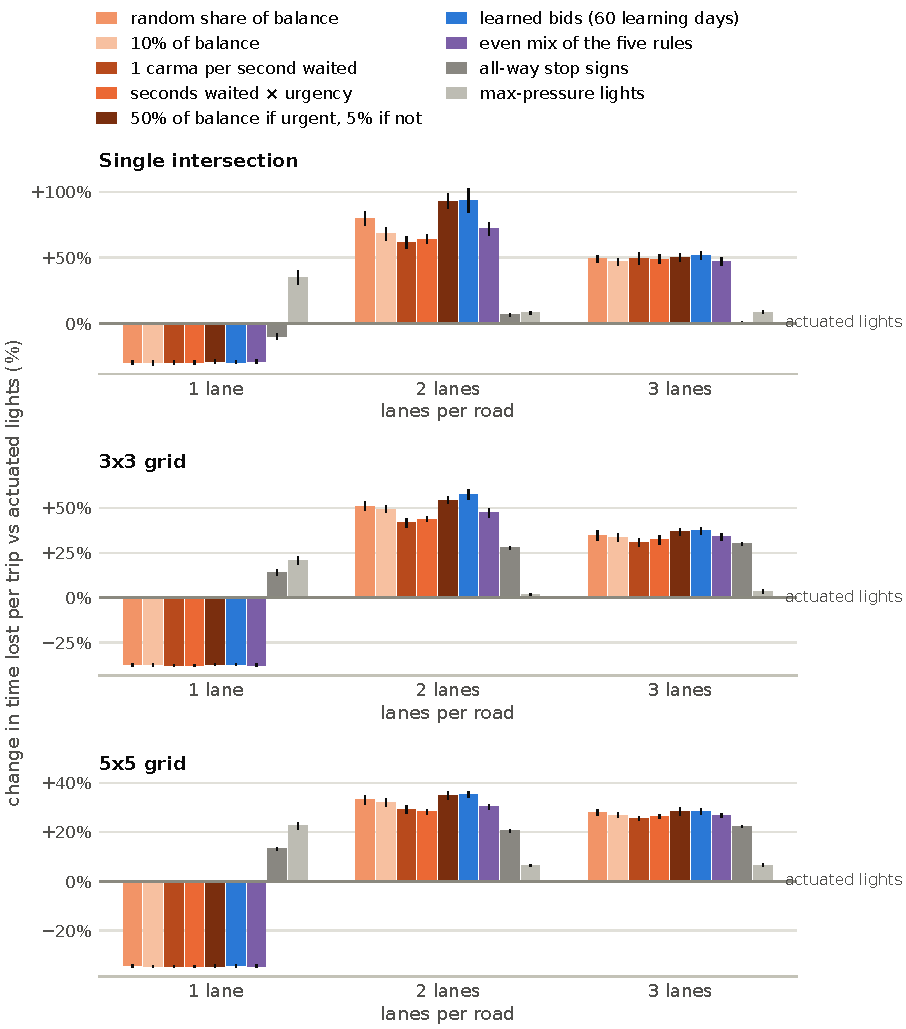
\includegraphics[width=\linewidth]{fixed_rules_time_lost.pdf}
    \caption{Time lost per trip under each fixed bidding rule, learned bids, an even mix of the
    five rules, stop signs and max-pressure lights, compared with actuated lights (0\%) on the
    same trips. Reference setting (moderate demand, 6 trips per driver, 20\% urgent trips, lane
    bids, 80 starting carma); fixed rules after 7 warm-up days and learned bids after 60
    learning days, then the same 7-day evaluation week; bars are means of 10 seeds of the
    paired difference, whiskers 95\% intervals; each panel has its own scale.}
    \label{fig:fixed_rules_time_lost}
\end{figure}

\begin{figure}[H]
    \centering
    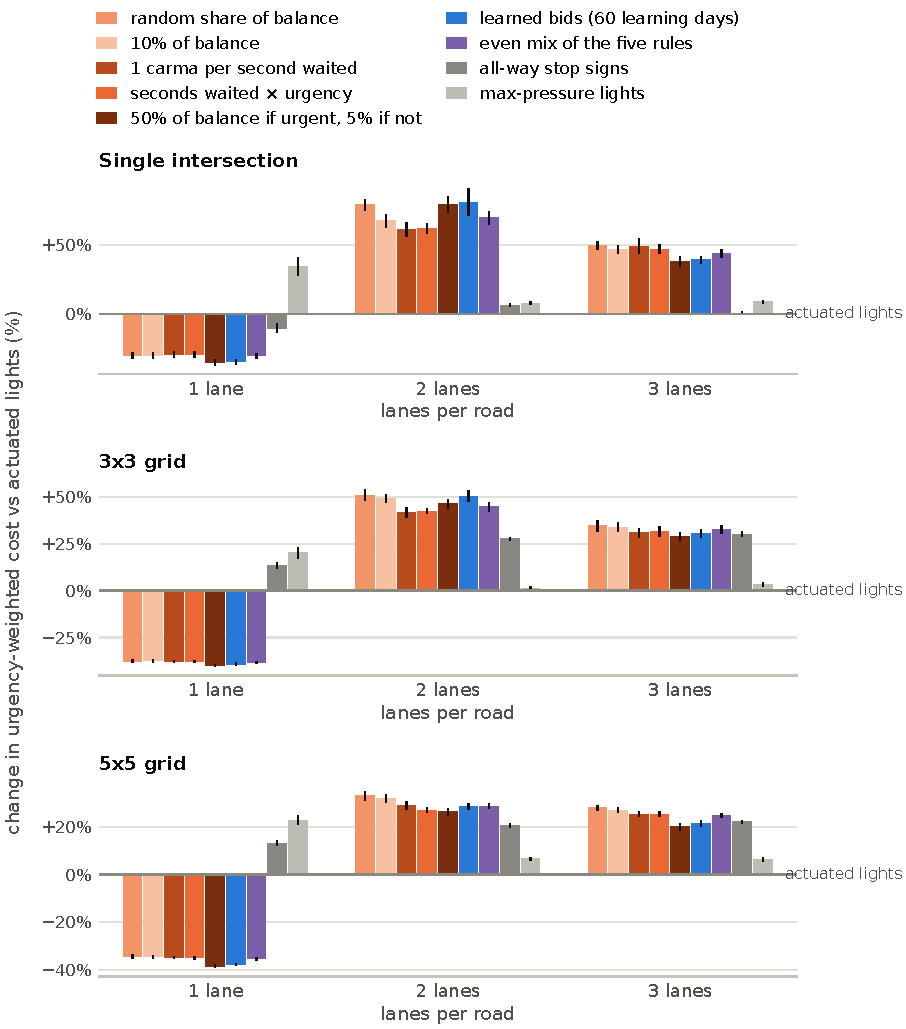
\includegraphics[width=\linewidth]{fixed_rules_cost.pdf}
    \caption{Urgency-weighted cost per trip (time lost $\times$ urgency, urgent trips weigh 6
    times calm ones), compared with actuated lights; settings as in
    Figure~\ref{fig:fixed_rules_time_lost}.}
    \label{fig:fixed_rules_cost}
\end{figure}

\begin{figure}[H]
    \centering
    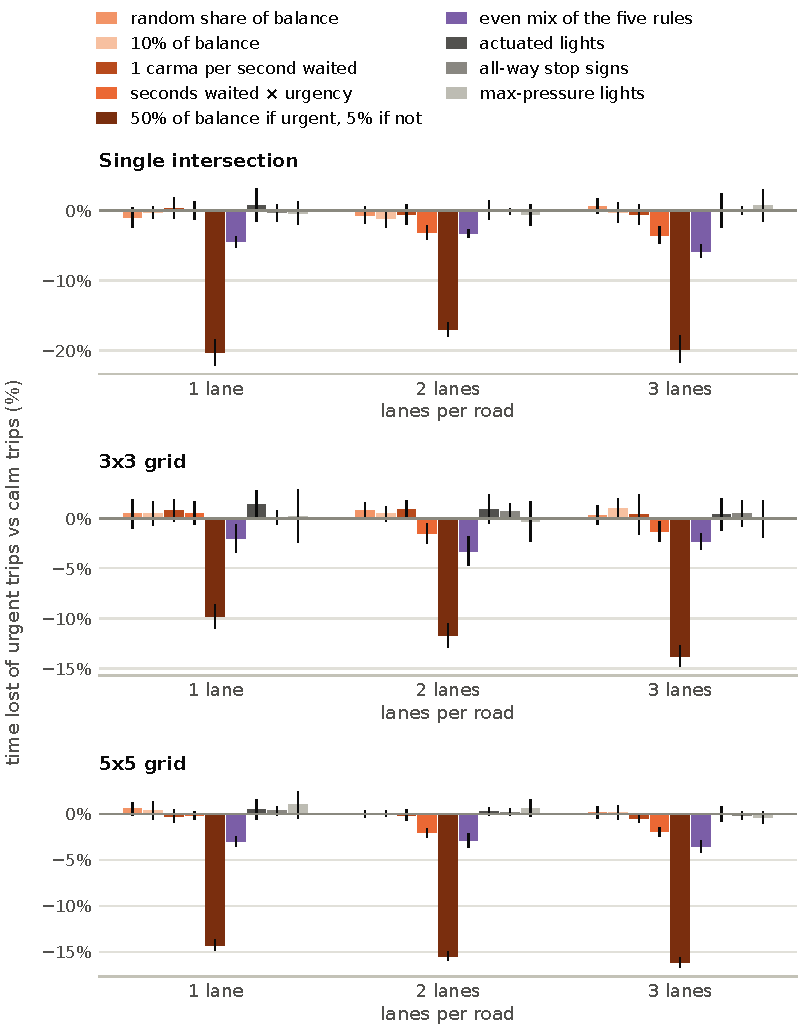
\includegraphics[width=\linewidth]{fixed_rules_urgency.pdf}
    \caption{How much less (negative) or more time urgent trips lose than calm ones under each
    rule; actuated lights, stop signs and max-pressure ignore urgency. Settings as in
    Figure~\ref{fig:fixed_rules_time_lost}.}
    \label{fig:fixed_rules_urgency}
\end{figure}

\begin{figure}[H]
    \centering
    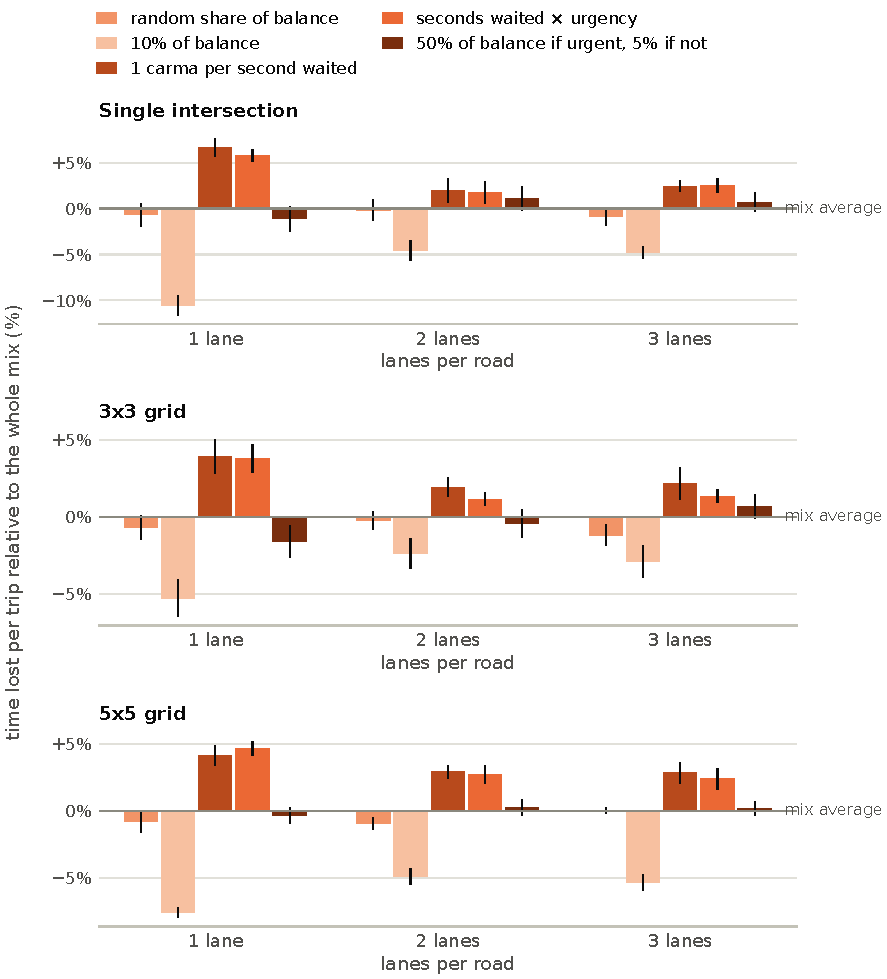
\includegraphics[width=\linewidth]{fixed_rules_mix.pdf}
    \caption{The even mix split by rule: time lost per trip of each rule's drivers relative to the
    whole mix, when every driver keeps one of the five rules (a fifth of the drivers each) and
    the car at the head of each lane bids by its own rule. Settings as in
    Figure~\ref{fig:fixed_rules_time_lost}.}
    \label{fig:fixed_rules_mix}
\end{figure}
